\documentclass{article}
\usepackage{times}
\usepackage{balance}
\usepackage{amssymb}
\usepackage{amsfonts}
\usepackage{amsmath}
\usepackage[amsmath,thmmarks]{ntheorem}
\usepackage{graphicx}
\usepackage{mathrsfs}
\usepackage{fancyhdr}
\usepackage{hyperref}

\graphicspath{ {Images/} }
\DeclareGraphicsExtensions{.pdf,.png,.jpg}

\DeclareMathOperator{\sgn}{sgn}

\newcommand{\R}{\mathbb{R}}
\newcommand{\C}{\mathbb{C}}
\newcommand{\Z}{\mathbb{Z}}
\newcommand{\id}{\textrm{id}}
\newcommand{\pr}{\mathrm{pr}}
\newcommand{\N}{\mathbb{N}}
\newcommand{\HRule}{\rule{\linewidth}{0.5mm}}


\newtheorem{thm}[equation]{Theorem}
\newtheorem{lem}[equation]{Lemma}
\newtheorem{prop}[equation]{Proposition}
\newtheorem{cor}[equation]{Corollary}
\newtheorem{conj}[equation]{Conjecture}

\theoremstyle{plain}
\theorembodyfont{\normalfont}
\newtheorem{defn}[equation]{Definition}
\newtheorem{ex}[equation]{Example}
\newtheorem{claim}[equation]{Claim}

\theoremstyle{nonumberplain}
\theoremheaderfont{\normalfont\bfseries}
\theorembodyfont{\normalfont}
\theoremsymbol{\ensuremath{\square}}
\theoremseparator{.}
\newtheorem{proof}{Proof}


\begin{document}
\begin{titlepage}
\begin{center}

% Upper part of the page. The '~' is needed because \\
% only works if a paragraph has started.

\includegraphics[width=0.2\textwidth]{./logo}~\\[1cm]

\textsc{\LARGE University of Copenhagen}\\[1.5cm]

\textsc{\Large StatML Exam}\\[0.5cm]

% Title
\HRule \\[0.4cm]
{ \huge \bfseries In a Galaxy Far, Far Away \\[0.4cm] }

\HRule \\[1.5cm]

% Author and supervisor
\begin{minipage}{0.45\textwidth}
\begin{flushleft} \large
\emph{Author:}\\
Alexander \textsc{Wahl-Rasmussen}
\end{flushleft}
\end{minipage}
\begin{minipage}{0.45\textwidth}
\begin{flushright} \large
\emph{KU Identity:} \\
\textsc{LGV740}
\end{flushright}
\end{minipage}

\vfill

% Bottom of the page
{\large \today}

\end{center}
\end{titlepage}
\pagestyle{fancy}
\lhead{}
\chead{\leftmark}
\rhead{}
\lfoot{Alexander Wahl-Rasmussen}
\cfoot{}
\rfoot{Page \thepage}

\section{Predicting the Specific Star Formation Rate}

\subsection{Linear Regression - Maximum Likelihood}

For this section I chose the Maximum Likelihood regression approach to do linear regression.
To solve the Maximum Likelihood, I first created a design matrix for the variables. 
I used a linear basis function of the form $\phi_i(x) = x_i$, and $\phi_0(x)$ = 1, so that it looks like the following : \medskip

\begin{equation} \label{eq:phi}
\Phi =
 \begin{pmatrix}
  1 & \phi_1(x1) & \cdots & \phi_{M-1}(x1) \\
  1 & \phi_1(x2) & \cdots & \phi_{M-1}(x2) \\
  \vdots  & \vdots  & \ddots & \vdots  \\
  1 & \phi_1(x_n) & \cdots & \phi_{M-1}(x_n) \\
 \end{pmatrix}
\end{equation}
\medskip

Where the first column marks the bias/offset parameter.

I then find the weight vector $w_{ML}$ by applying the following formula:
\medskip
\begin{equation} \label{eq:w}
w_{ML}=(\Phi^T \Phi)^{-1} \Phi^T t
\end{equation}
\medskip

I then use the variables from \eqref{eq:phi} and \eqref{eq:w} to predict the targeted values:
\begin{equation}
Y = w_{ML} * \Phi
\end{equation}


\noindent The results for the train and test set can be seen in Table \ref{table:linear}. 
Given that the Mean Squared Error can vary from 0 to infinity, with 0 being a perfect match and infinity being the worst possible match, the result we get seems quite good. 
It does indeed seem like we can approximate the logarithm of the sSFR with a linear regression. 
It is also worth noting that the error rate is low for both the train and test set which seems to indicate that both datasets have the same degree of noise and belong to the same domain, i.e. the data we learn on can be considered ``typical'' samples.  


\begin{table}[htb]
\centering
\caption{Non-Linear Regression Results}
\label{table:linear}
\begin{tabular}{l|c}
	\hline \hline
	Train Mean Squared Error & 0.2748 \\
	Test Mean Squared Error & 0.2752 \\
\end{tabular}
\end{table}

\subsection{Non-Linear Regression - Maximum A Posteriori}

For the non-linear regression I chose the Maximum A Posteriori regression approach instead.
I used the formulae:
$m_N = \beta S_N\Phi^T t$ for the mean and $S^{-1}_N = \alpha I + \beta \Phi^T\Phi$ for the covariance.
I assigned the noise precision parameter $\beta$ to 1, and set the range of $\alpha$ between 0 and 10, in increments of 0.5, wnere alpha can be considered the regularization parameter.
Additionally, I chose a polynomial regression with the power varying from 2 to 5. 
I limited the power as to prevent overfitting by creating a complex model with a high power that only fits the presented data.
The choice of maximum 5 is due to each data point only having 4 dimensions meaning any higher power would lead to poor generalization.

To find the optimal parameters I then perform a gridsearch of the two parameters, power \& $\alpha$, combined with a 5-fold crossvalidation on the train set.
The crossvalidation then returns the parameter pair that yields the lowest average test error on the train set. 
I then use those parameters to train on the entire train set, test on both the train and test set, and the Mean Squared Error can be seen in Table \ref{table:non-linear}

\begin{table}[htb]
\centering
\caption{Non-Linear Regression Results}
\label{table:non-linear}
\begin{tabular}{l|c}
	\hline \hline
	$\alpha$ & 9.5 \\
	Power & 3 \\
	Train Mean Squared Error & 0.1698 \\
	Test Mean Squared Error & 0.1911 \\
\end{tabular}
\end{table}

\section{Stars vs. Galaxies}

\subsection{Binary Classification with Support Vector Machines}


For this section I used the the \textit{SVC}\cite{website:svm-sklearn} function, which is a SVM implementation that is based off the LIBSVM \cite{website:libsvm} library.
The mathematical formulation of the learning problem it tries to satisfy is given in \cite[1.2.7.1. SVC]{website:svm-sklearn}, with the decision function being:

\begin{equation} \label{svm}
\sgn{(\sum_{i=1}^n y_i \alpha_i K(x_i,x) + p)}
\end{equation}
where $y_i\alpha_i$ is the dual coefficients for the support vectors and p an individual constant term \footnote{For a more in-depth explanation of how the SVM works, see section 3.1 where I explain the classifier. In that example the SVM has a linear kernel, but the method is the same.}.

The kernel in this case is radial of the form $k(x,x') = \exp{ (-\gamma || x - x' ||^2) }$, where the relevant hyperparamters are the influence term $\gamma$ and the margin paramter C. For a high $\gamma$ we reduce the influence radius of each data point while a low value will increase its influence.
Likewise, a high value for C will enforce a hard margin where every train example will be classified correctly, while a small value will make the decision boundary more smooth with more errors on the train set.
This means having a high value of C might not be wanted, because it can result in overfitting and therefore subpar generalization. 

To achieve good results and an efficient solution I again normalized the data with zero mean and unit variance.
Unlike for the K-means I did not do it to increase the performance of the classifier as such, but to reduce the training time. 
My approach was first to sample the $\gamma_Jaakkola$ constant from the entire dataset and then do a gridsearch for $\gamma$ and $C$ combined with a 5-fold crossvalidation on the trainset while averaging over the crossvalidate-train and crossvalidate-test errors.
I chose to extend the range of $\gamma$ to also include $b^-4$ and $b^4$ with b being eulers number. 


%The sigma_jaakkola is:  1.01805438506
%The y_jaakkola is:  0.482423046115

%Best hyperparameter (C, gamma):  (20.085536923187668, 0.0240184291791639)
%Train Loss: 0.005500 , Test Loss: 0.006000
%RBF SVM Loss on train:  0.00533333333333
%RBF SVM Loss on test:  0.005


\subsection{Principal Components Analysis}

For PCA I used the approach given in \cite[pp. 561-563]{bishop}, which is the maximum variance method. 
This means that I first sample the mean and variance from the dataset that corresponds to the galaxies. 
I then normalize the data with zero-mean and unit variance, not because it is requried for PCA or improves the performance, but because it improves the clustering performance in the next section.
More on that there.
I then resample the mean and the covariance matrix from the normalized distribution, where I compute the eigenvectors of the covariance matrix.
The eigenvectors corresponds to the principal components of the distribution, where the eigenspectrum is plotted in Figure\ref{fig:eigen}.
The low eigenvalues are due to normalization.
I then project the data onto the two principal components with the highest eigenvalues by computing the dot product between the eigenvectors and the data points, where the eigenvectors are row vectors and the data points are vectors.
The scatter plot of the dimensionality reduced data points can be seen in Figure\ref{fig:projecting}

\begin{figure}[htb]
\centering
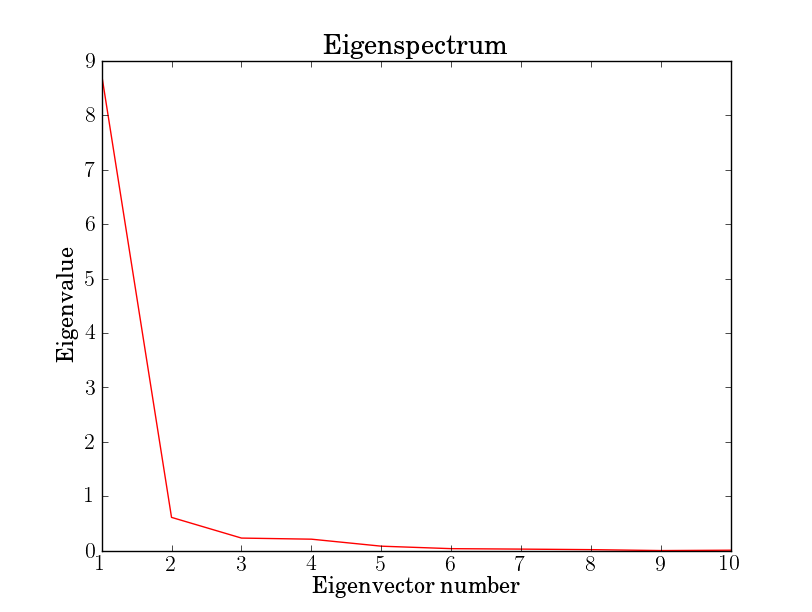
\includegraphics[height=5cm]{Images/eigenspectrum.png}
\caption{Eigenspectrum of the normalized SGData}
\label{fig:eigen}
\end{figure}


\begin{figure}[hbt]
\centering
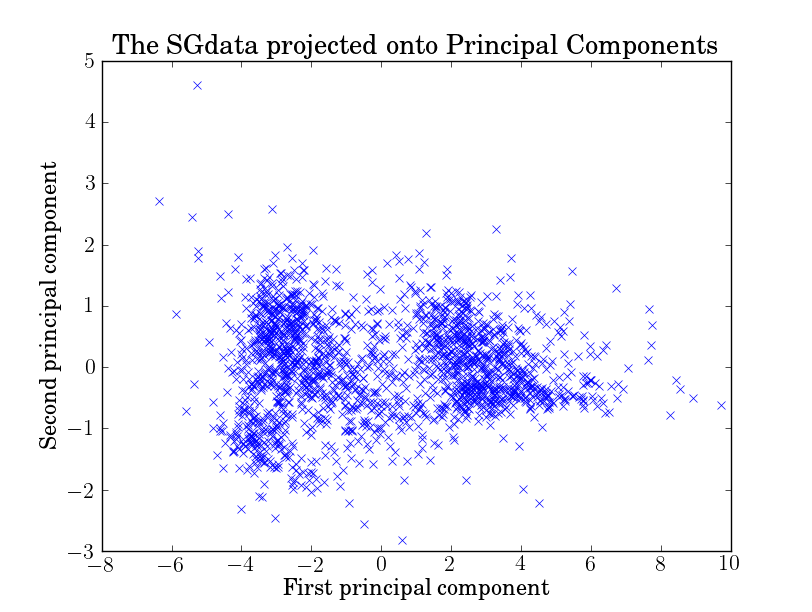
\includegraphics[height=5cm]{Images/PCA_scatter.png}
\caption{Projecting of the normalized data onto the 2 first Principal Components}
\label{fig:projecting}
\end{figure}


\subsection{Clustering}

For this section i chose the K-means implementaion from the Scikit-Learn library \cite{website:kmeans}. 
The K-means classifier is an unsupervised learning methods, meaning that it classifies by finding a hidden structure in the data that it tries to extracct. 
It runs on unlabeled data meaning we have no exact way of measuring its error besides the judgement of our own interpretation. 
Specifically, the K-means clustering algorithm tries to sort the data into K clusters by minimizing the within cluster sum of square objective function. 
The mathematical formulation of this function, for a dataset X with n samples, is:

\begin{equation} \label{km}
J(X,C) = \sum_{i=0}^n \min_{u_j \in C}(||x_j - \mu_i||^2)
\end{equation}

As is seen in the equation, the function relies on the Euclidean distance, which performs best on normalized data.
This is due to the distances between the data points with higher value ranges will be over-emphasised, i.e. the distance will seem bigger than (relatively) they are.
Therefore I took the liberty of normalizing the data by zero mean and unit variance, which of course affects the location of the mean. 

The algorithm itself runs in 3 steps.
The first step is the initialization of the centroids, and in this case they are chosen at random. 
Step two is assigning every data point to its nearest mean with equation~\eqref{km}. 
Step three is measuring the difference between the old mean and the new mean.
Step two and three are then repeated untill the difference value is less than the threshold of 0.0001 or the maximum number of iterations have been reached (300). 

After the two centroids have been located I project them with the same projection as in the previous section.
The plot can be seen in Figure \ref{fig:kmeans} and the Table \ref{table:centroid}. 

As for the placement of the centroids they seem quite intuitive.
We almost see a white diagonal `decision boundary' in the data around starting at (-2,5) and ending in (4,-3), which makes the centroid location even more plausible.
As this is an unsupervised classification I have labels to measure the classification up again, so to truly answer the question it would require additional knowledge of galaxies, which I sadly do not have. 
According to the plot however, it seems meaningful. 

\begin{table}[h!]
\centering
\caption{Centroid Coordinates}
\label{table:centroid}
\begin{tabular}{l|cc}
	\hline \hline
	First Centroid & -2.476 & -0.032 \\
	Second Centroid & 2.835 & 0.036 \\
\end{tabular}
\end{table}

\begin{figure}[htb]
\centering
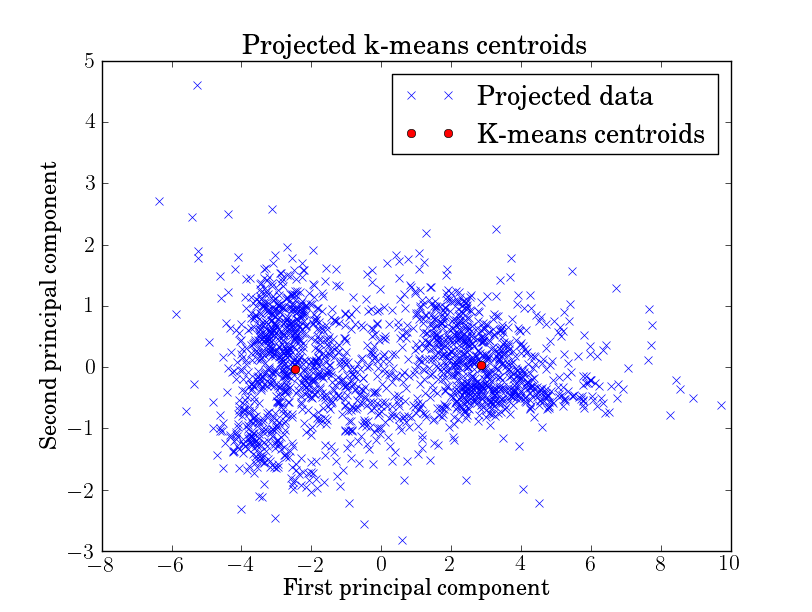
\includegraphics[height=5cm]{Images/Kmeans_PCA.png}
\caption{The centroids and data points projected onto the 2 Principal Components}
\label{fig:kmeans}
\end{figure}

\subsection{Kernel Mean Classifier}

\begin{claim}
This is really fun!
\end{claim}

\begin{proof}
Since
\begin{equation} \label{eq2}
a + b + c = d
\end{equation}
it follows that equation~\eqref{km} is a fun equation.
\end{proof}

\section{Variable Stars}

\subsection{Multi-Class Classification}

For this part I chose two classifiers with K-NearestNeighbor (KNN) as my non-linear, non-parametric classifier and Support Vector Machine with a linear kernel (SVM) as my linear, parametric classifier.
Both learns with supervised learning.
There are several reasons for why I chose these classifier and why I consider a SVM with a linear kernel as a linear classifier, as shall now become evident.
However, let us start by examining how the algorithms classify.
Imagine a case, where we only have 3 samples and 2 categories, in a n-dimensional space, and the first sample belongs to the first class while the second sample belongs to the other category.
We then want to classify the third sample based on its features compared to the classified samples' features. This means we first train the specific algorithm on the two samples and then run the algorithm on the last sample. \medskip

The \textit{(K-)NN} will then try to find the nearest neighbour by calculating the distance between the test sample and all other training data points. The nearest neighbour will then be the training data point that has the shortest distance to the test data point. The test data point is then classified as having the same class as its nearest neighbour, because their features are most alike.
The amount of nearest neighbors to be considered can be increased and this notated with a K - hence the name KNN, where the classification decision is based on majority voting between the neighbors. 
The distance metric itself can also vary, e.g. it can either be Euclidean, Manhattan, Hamming etc., where the three also are known as direct, absolute and binary distances.

A \textit{Linear SVM} will instead try to create a linear spatial decision boundary (in this case a straight line). The data is then divided   . This resembles the approach of the Perceptron, but instead of trying to minimize the amount of errors, it creates the decision boundary at the maximum distance from the nearest data points, which is also known as the support vectors. So instead of finding \textit{a} decision boundary it tries to the \textit{the best} decision boundary.
Intuitively this also means that the bigger the distance (or margin) is to the nearest support vectors, the lower amount of prediction errors should be.
It should be noted that having a hard margin may not be ideal, since it can result in overfitting on the train set, which leads  to bad generalizations.
Unlike Perceptron, the linear SVM can also classify non-linear distributions by utilizing the ``kernel trick'' and projecting the distribution into an unknown, but well-defined, high-dimensional space. In this space the distribution will then become linearly seperable and the decision boundary can be located.
The kernel itself can also be changed to a non-linear function such as we have seen in chapter 2.1.
I have simply run the linear SVM, which can arguably be described as a conceptual extension of the Perceptron. \medskip


The reason why I included the descriptions of the algorithms is quite simple: I believe that one of the biggest strengths of both classifiers is how they classify. 
That is, their approach to classification is very intuitive.
It makes sense that the within class data should ``look alike'' and have a short distance to eachother in the Euclidean space.
It also makes perfect sense, that we should care about finding the \textit{best} decision boundary, which is what SVM tries to do. 

Furthermore, if I had used another linear classifer, such as the Perceptron, and had the dataset not been linearly seperable in its current form I would have had to make certain decisions.
Would I want to stop the Perceptron at a certain iteration, which is a quite common approach\footnote{Even the Scikit-Learn has a max iteration declared as a default!}, and if so, what iteration would I choose?
Alternatively, I could have reduced the dimensions with PCA, or increased it with additional information such as the distance to the mean, to find the optimal dimension where the data is linearly seperable. 
But why go through such hassle of finding the optimal dimensions when I can utilize the kernel trick to do the exact same thing without actually computing it.

So while it very well can be argued that a linear SVM is neither a linear classifier, since it does not linearly seperate the data in the given space, nor a multi-class classifier, I believe that the steps you would otherwise take would result in almost the same approach. 


\subsubsection{Description of software used}
For both classifiers I used implementaions from the Scikit-Learn Python library\cite{website:sklearn}. \medskip

The \textit{KNeighborsClassifier} is a KNN implementation that also incorporates an underlying data-structuring algorithm such as a KDTree, Ball Tree or `brute force'\cite{website:knn-sklearn}. 
The brute force search is the `vanilla' KNN where every data point is iterated over, while both KDTree and Ball Tree partitions the data into trees, where the KNN algorithm then iterates over the tree nodes instead.
Any re-structuring of the data will of course affect the performance and the decision-making of the classifier, where the impact on the former is much higher than the latter. 
However, as I have a fairly limited knowledge of space-partitioning, I chose the beautiful setting of `auto', where the function itself chooses an appropriate algorithm parameter as to achieve the most efficient solution. The only parameter I then have to supply is the amount of neighbors K. Additionally, the function .score(X,y) returns the accuracy instead of the 1-0 Loss and this I manually convert with $Loss = 1 - Accuracy$. \medskip

The \textit{SVC}\cite{website:svm-sklearn} is a SVM implementation that is based off the LIBSVM \cite{website:libsvm} library. 
It is the same implementation as the one in section 2.1 with the same decision function \eqref{svm}. 
As the SVM is a binary classifier it employs a one-by-one strategy for multiclass classification. This means that the function creates one classifier per class-pair, meaning the class with most votes among the subsets is chosen
\footnote[1]{This means that for a case of n classes there will be a classifier for each pair: 0 vs 1, 0 vs 2, .. 0 vs n, 1 vs 2, .. n-1 vs n}.
This is in contrast to the one-vs-all implementation, where each class is matched against the rest of the classes. I also chose the output to be deterministic and with the class weight set to 1, meaning each class has the same weight. Furthermore, the function .score(X,y) returns the accuracy  which I then convert to a 0-1 loss.

\subsubsection{Results}
To achieve the best results I first normalized the data by making it zero-mean with unit variance as I explained in the previous sections.
I chose to normalize my data for two reasons. 
Since KNN matches by minimum distances it inherently assumes that all our data has the same range of values, which means that distances between the data points with higher value ranges will be over-emphasised. This can be avoided by normalizing. 
SVM does not explicitly suffer from this problem since it only considers the support vectors and not the entire dataset. 
But due to its bad scaling behaviour it improves the training time to reduce the value range and it forces both classifiers to perform on equal footing.
I then perform a 5-fold crossvalidation on the train set to find the optimal parameters K and C.
K is a list of integers between 1 \& 15 and C is a list numbers from 0.005 to 1 with step size 0.005. 
Initially I also tested $C_i > 1$ but that did not increase the test result, which results in a soft margin.
I then return the parameters that gave the lowest average test loss.
The results from the \textit{entire} train and test set can be seen below. 
To see the results of the crossvalidation you will have to run the code.

\begin{table}[h!]
\centering
\caption{Multi-Class Classification Results}
\label{table:multiclass}
\begin{tabular}{ l | l  l  l }
	\hline \hline
  Classifier & Hyperparameter & Train Error & Test Error \\ [0.5ex]
  	\hline
  KNN & K = 8 & 0.280 & 0.341 \\
  Linear SVM & C = 0.06 & 0.147 & 0.265 \\
  \hline
\end{tabular}
\end{table}

At first glance the results does not seem very impressive.
But, if we consider that each data point has 61 features and can belong to one of 25 different classes \textit{and} that there's only 771 training and equally many test samples, the results does not seem that shabby. 
Usually you would want a 80/20 or even 90/10 split between train and test size as to achieve good results.
It is therefore not too surprising that the results do not reach a lower error rate.
That is even without considering the sparsity of the dataset compared to the dimensionality of each datapoint.
And that class 2 only has 1 data point! This means KNN will never classify it correctly. 
The sparsity will also affect the crossvalidation negatively, since some classes might be absent from one or more folds, which would lead to a poorer performance. 
The relatively high value of K and low value of C also indicates that the data is quite noisy, which again also reduces the performance of the crossvalidation.
However, I do not think splitting the train set into a train/validate test set would prove any better due to the sparsity of the data.

It is also worth noting that my knowledge of the relationship between machine learning and star-detection is quite limited.
Therefore I can not relate the results to any other experiments regarding the same dataset. 
Simply put: I have no idea if this is even close to competitive results, but I know that it is at least much better than a random cointoss! 
As to improve on the results, it might be beneficial to reduce the dimensionality with e.g. PCA to diminish the amount of noisy dimensions.

\subsection{Overfitting}




\bibliographystyle{acm}
\bibliography{biblo}

\end{document}